\chapter*{decay}
\addcontentsline{toc}{chapter}{decay}
\begin{center}
\vspace{2cm}
\begin{flushright}
\large
\textit{ $n \rightarrow p^+ + e^- + \bar{\nu}_e$ }
\end{flushright}
\vspace{2cm}
% \vspace*{\fill}
\end{center}
\normalsize

\newpage  % Move to the next page
Decay is a fundamental process of transformation, marking the passage from one state of existence to another. In the realm of particle physics, when an atom has an unstable configuration, such as an excess of neutrons, it undergoes decay to achieve stability. A neutron transforms into a proton, emitting an electron and an antineutrino in the process, in a phenomenon known as beta-minus decay.

%% image
\begin{figure}
    \centering
    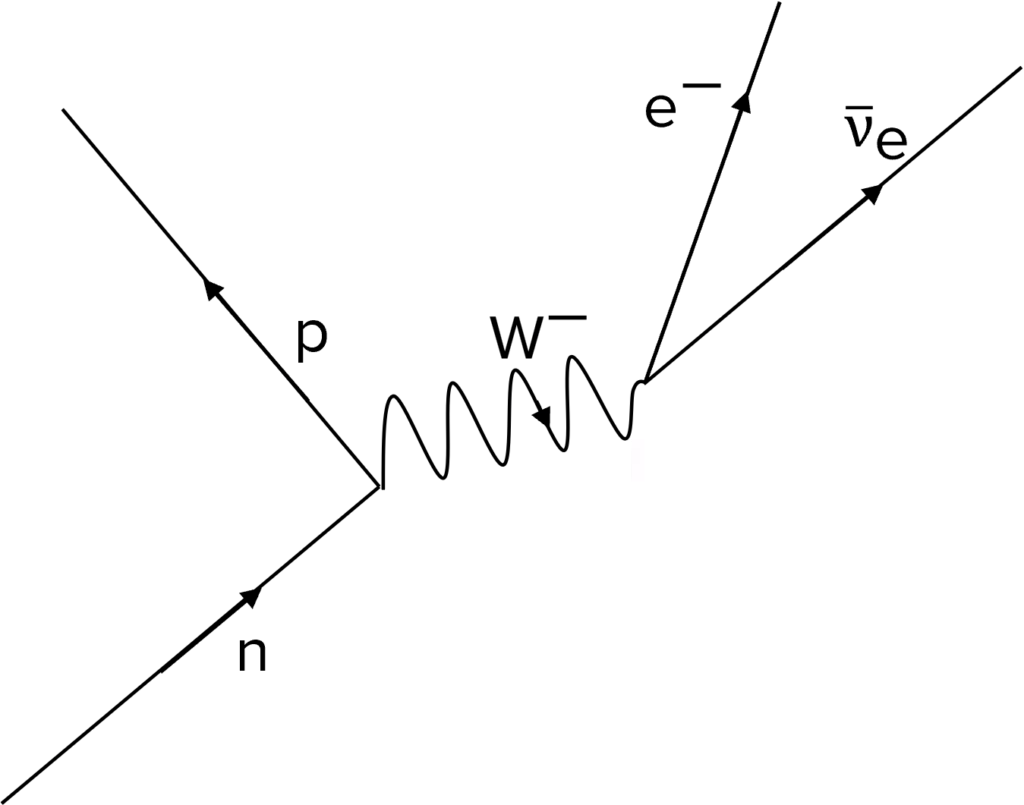
\includegraphics[width=0.8\linewidth]{assets/betaminusdecay.png} 
    \caption{\small Beta-minus decay.}
    \label{fig:betaminusdecay}
\end{figure}

Just as the carbon-14 that undergoes radioactive decay over millennia, serving as a measure of time and history, our lives too are governed by the forces of transformation and impermanence. The weight of indecision, uncertainty, and imbalance manifests as forces propelling us toward change. And like the remaining stable nitrogen-14, we seek equilibrium, a resolution to the chaos that defines our existence. Much like the emitted radiation observed in atomic reactions, the disruptions and losses we experience are the byproducts of our transformation.

Everything is transient, every present moment unfolds from the past. Processes of becoming and unbecoming underscore the interconnectedness of all phenomena. The second law of thermodynamics shows a universe driven toward higher entropy, defining the arrow of time. This entropy is not merely a measure of chaos but a sign of the potential for transformation. Decay is a precondition for creation.

In the digital realm, decay mirrors the entropic nature of information and memory. Glitches, data loss, and the degradation of digital media are reminders of the fragility of permanence in a system that relies on energy and maintenance. Artists and technologists alike have explored the concept of digital decay, creating dynamic pieces designed to purposefully degrade and transform over time. These works challenge the idea of art as a static entity, taking advantage of the beauty of impermanence.

% note: glitch ?

Dieter Roth’s  (1930-1998) artistic practice is deeply linked to the theme of decay, both conceptually and materially. His work explores impermanence, transformation, and the natural processes of deterioration, challenging traditional notions of art as something static or preserved. Roth famously incorporated rotting foodstuffs such as cheese, chocolate, and bread into his sculptures and installations. These materials naturally decomposed over time. His biodegradable artworks were never meant to remain in a fixed state, making decay an essential part of their existence rather than an unintended consequence. Instead of seeing decay as destruction, Roth embraced it as a creative force. Works like "Insel" (1968), or "Small Landscape" (1969) which combined food with other materials, allowed the viewer to witness changes in texture, color, and form over time. This made entropy and organic breakdown an integral part of the viewing experience. See figure ~\ref{fig:roth}.


%% image
\begin{figure}
    \centering
    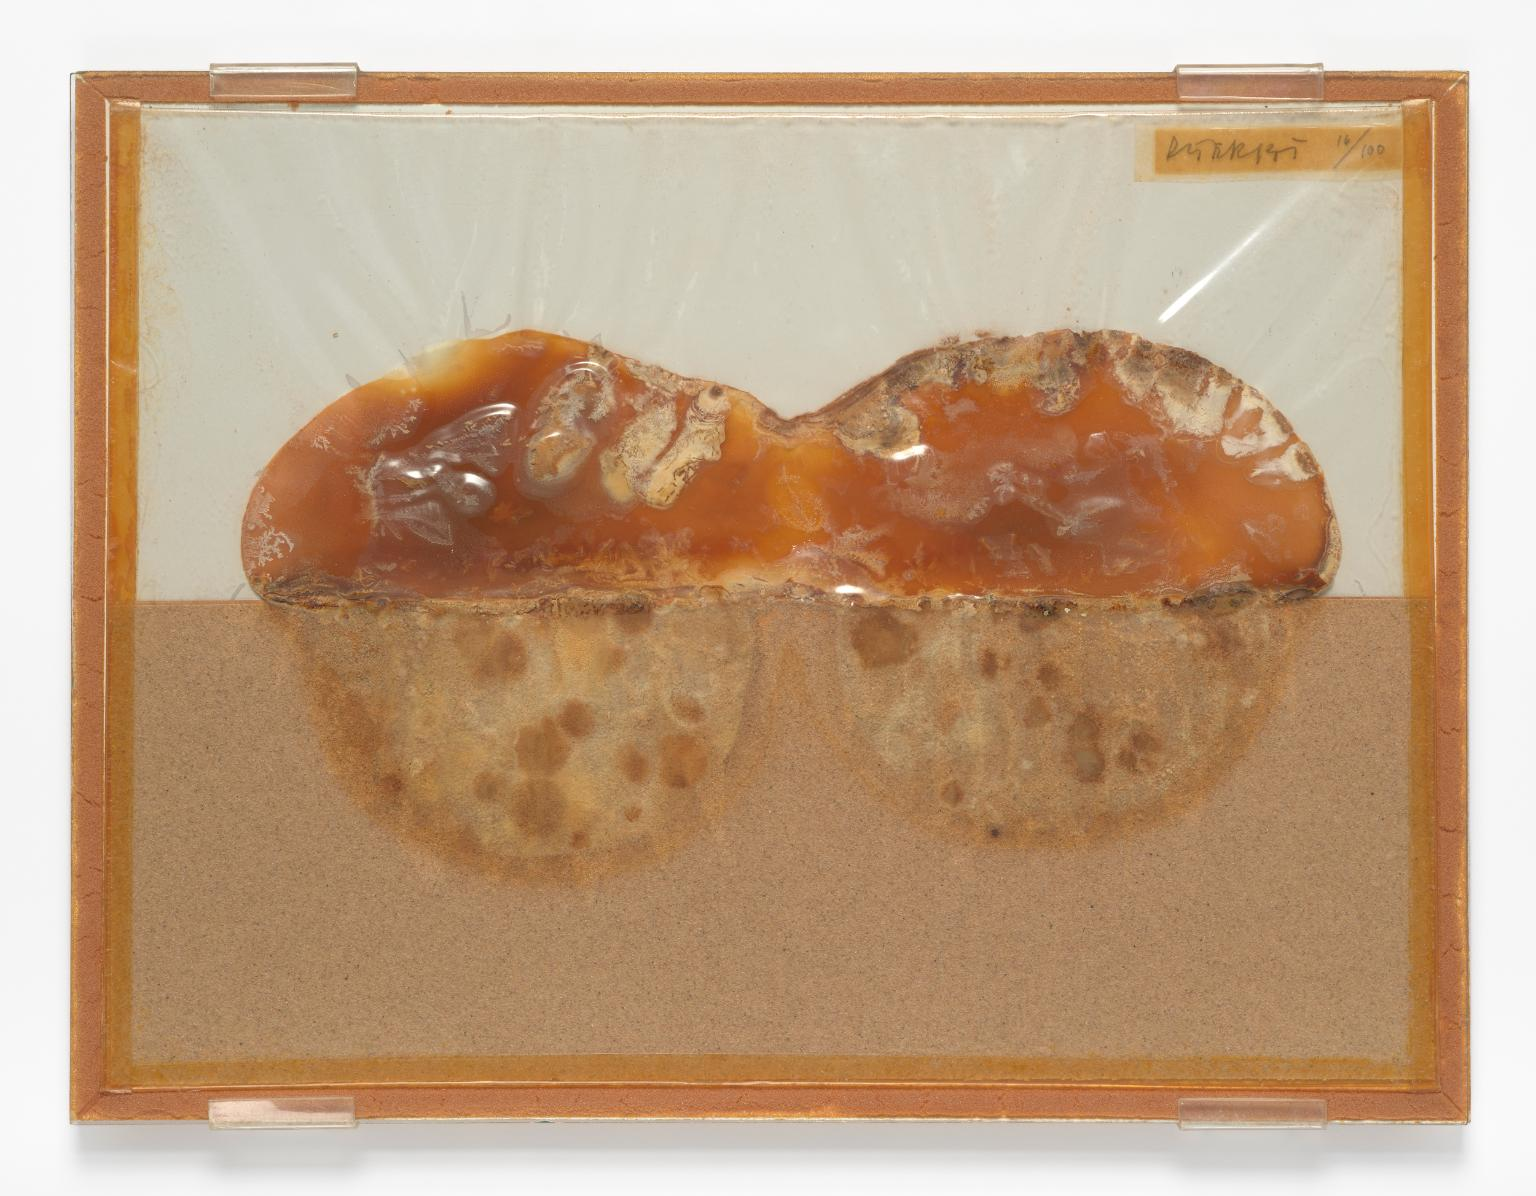
\includegraphics[width=0.8\linewidth]{assets/roth.jpg} 
    \caption{\small Small Landscape - \textit{Dieter Roth , 1969, https://www.tate-images.com}.}
    \label{fig:roth}
\end{figure}

Traditional art forms aim for preservation, but this rigid approach can be altered by creating artworks that could not last. Deteriorating sculptures and digital media meant to be corrupted defies the idea of museums and galleries as places of eternal conservation, forcing audiences to confront the reality of time and change. In many traditions, the impermanence of materials serves as a reminder of our ephemeral nature, that no matter how strong, beautiful, or lasting something appears, it is subject to the forces of time.

% note: add images from roth work
Often viewed through the lens of entropy as a gradual decline into disorder, decay also serve as a powerful symbol for mortality and impermanence, reflecting the fundamental nature of existence, both human and material. Transient and ever-changing. Across philosophy, art, and science, these processes of breakdown also represent transformation, renewal, and continuity. They mirror the human experience of aging and illness, a reminder of death, highlighting the inevitable dissolution of the body and mind over time, challenging the idea of fixed identities. 

% The Disintegration Loops is a series of four albums by the American avant-garde composer William Basinski,
% https://en.wikipedia.org/wiki/The_Disintegration_Loops

% note : use this example... dementia ---

% Everywhere at the End of Time[a] (commonly shortened to EATEOT) is the eleventh recording by the Caretaker, an alias of English electronic musician Leyland Kirby. Released between 2016 and 2019, its six studio albums use degrading loops of sampled ballroom music to portray the progression of dementia and related neurological conditions
% https://en.wikipedia.org/wiki/Everywhere_at_the_End_of_Time


% note: art or culture for that matter represent 'negentropy': an effort to fight against the tendency of collapse .

Decay, as the physical consequence of \textit{decadence}, carries an undeniable aesthetic and emotional weight. The textures of rusting metal, peeling paint, or decomposing wood evoke a melancholic beauty, resonating with human emotions of nostalgia and loss. This attraction to decay (\textit{ruin lust}) reveals an innate fascination with the traces of time left on objects, places, and bodies.

The 19th-century Decadent movement in literature and art, for example, was fascinated by fading beauty, decline, and the grotesque. Writers like Joris-Karl Huysmans explored themes of decay, (e.g. \textit{"À rebours"}, 1884) intoxication, and exhaustion, seeing ruins, disease, and corruption as sources of strange and melancholic beauty. \citep{huysmans1884}. In "À rebours", Huysman depicts Des Esseintes, an aristocrat who retreats from society into an isolated world of extreme aesthetic indulgence, rejecting conventional morality, nature, and human interaction in favor of artificial beauty, refined pleasures, and self-destructive excess. 

The idea of replacing reality with artificial experiences, surrounding himself with refined art, literature, and intoxicating sensory stimuli is not foreign to our current technologically oriented era. It mirrors how today's society curates reality through digital technology, consuming endless streams of algorithmically personalized content on social media, entertainment platforms, and virtual spaces. Platforms like Instagram, TikTok, and YouTube create hyper-aestheticized, exaggerated versions of life, much like the way Des Esseintes surrounded himself with extreme beauty. This leads to an artificial sense of fulfillment but ultimately disconnects users from genuine human experiences, through instant gratification and dopamine loops.

One of the most striking aspects of Against the Grain is the character's withdrawal from real-world human interaction in favor of a self-constructed, idealized environment. Similarly, technology has made it easier for people to disconnect from face-to-face interactions, replacing them with digital relationships, parasocial bonds, and algorithmic companionship. Social media and digital avatars allow individuals to construct idealized versions of themselves, obsessively controlling our surroundings. Yet this perfectionism leads to anxiety, burnout, and a sense of inauthenticity.

Serving as both an end and a beginning, decay is the dissolution of what was and the emergence of what could be. In embracing decay, we accept the inevitability of change and the transformative power it holds. Whether in the disintegration of memory or the breakdown of stability, decay serves as an excuse to find value and meaning in impermanence.


% outro

The closed door at the end of the corridor has always been there, as an object of curiosity, an anchor for fear, a boundary between the known and the speculative. This thesis has explored the structures of cognition, the unpredictability of perception, and the resistance against deterministic narratives. I attempted, through my own lense, to draw parallels between neurodivergence and systems of knowledge, between artistic creation and scientific inquiry, between the physical constraints of space and the abstract dimensions of thought. Based on the fragmented nature of time and memory, the recursivity of perception and an ongoing negotiation of identity, I have attempted to weave together theory and experience. This text is not a closed system; it is an invitation to further exploration. 